\section{End Flag Generator}

To generate a valid \(END\_FLAG\) signal for the ALU, a Timed Mealy State Machine is introduced into the circuit.
The ASMD charts of the 1 stage and 4 stages \(END\_FLAG\) generator are presented in \figref{fig:asmd}.
% And the RTL description of the 4 stages \(END\_FLAG\) generator is presented in \figref{fig:end_flag_gen_rtl}.

For pipelined circuit, the \(END\_FLAG\) will result in the output after counting 4 synchronized clock cycles
when the \(LOAD\) signal goes from high to low. The counting of the clock cycle is implemented by rotating a
vector signal to avoid introducing an extra addition circuit.

For non-pipelined circuit, the \(END\_FLAG\) will result in the output of a clock later after the \(LOAD\) signal goes from high to low.

\begin{figure}[!ht]
	\centering
	\caption{ASMD Chart of the FSM of Different End Flag Generator}
	\label{fig:asmd}

	\subfloat[1 Stage \(End\_Flag\) Generator]{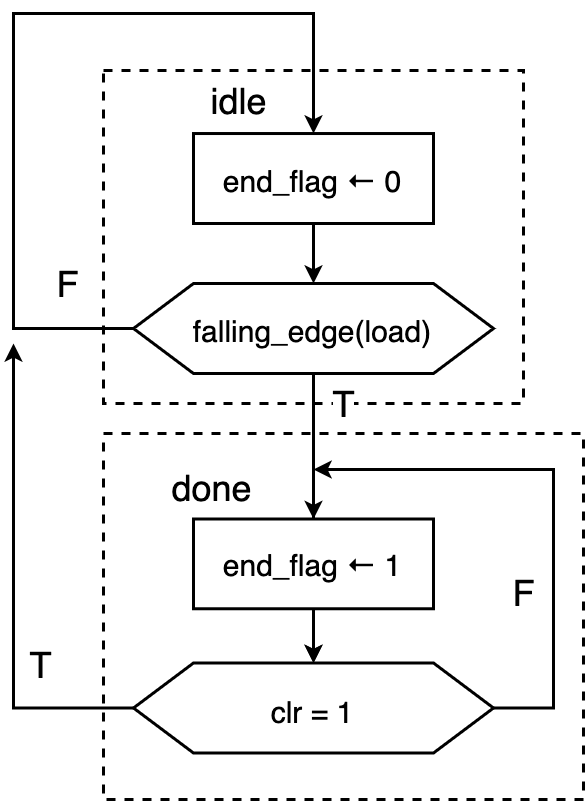
\includegraphics[width=0.3\textwidth]{./img/asmd_2.png}}
	\hspace{1cm}
	\subfloat[4 Stages \(End\_Flag\) Generator]{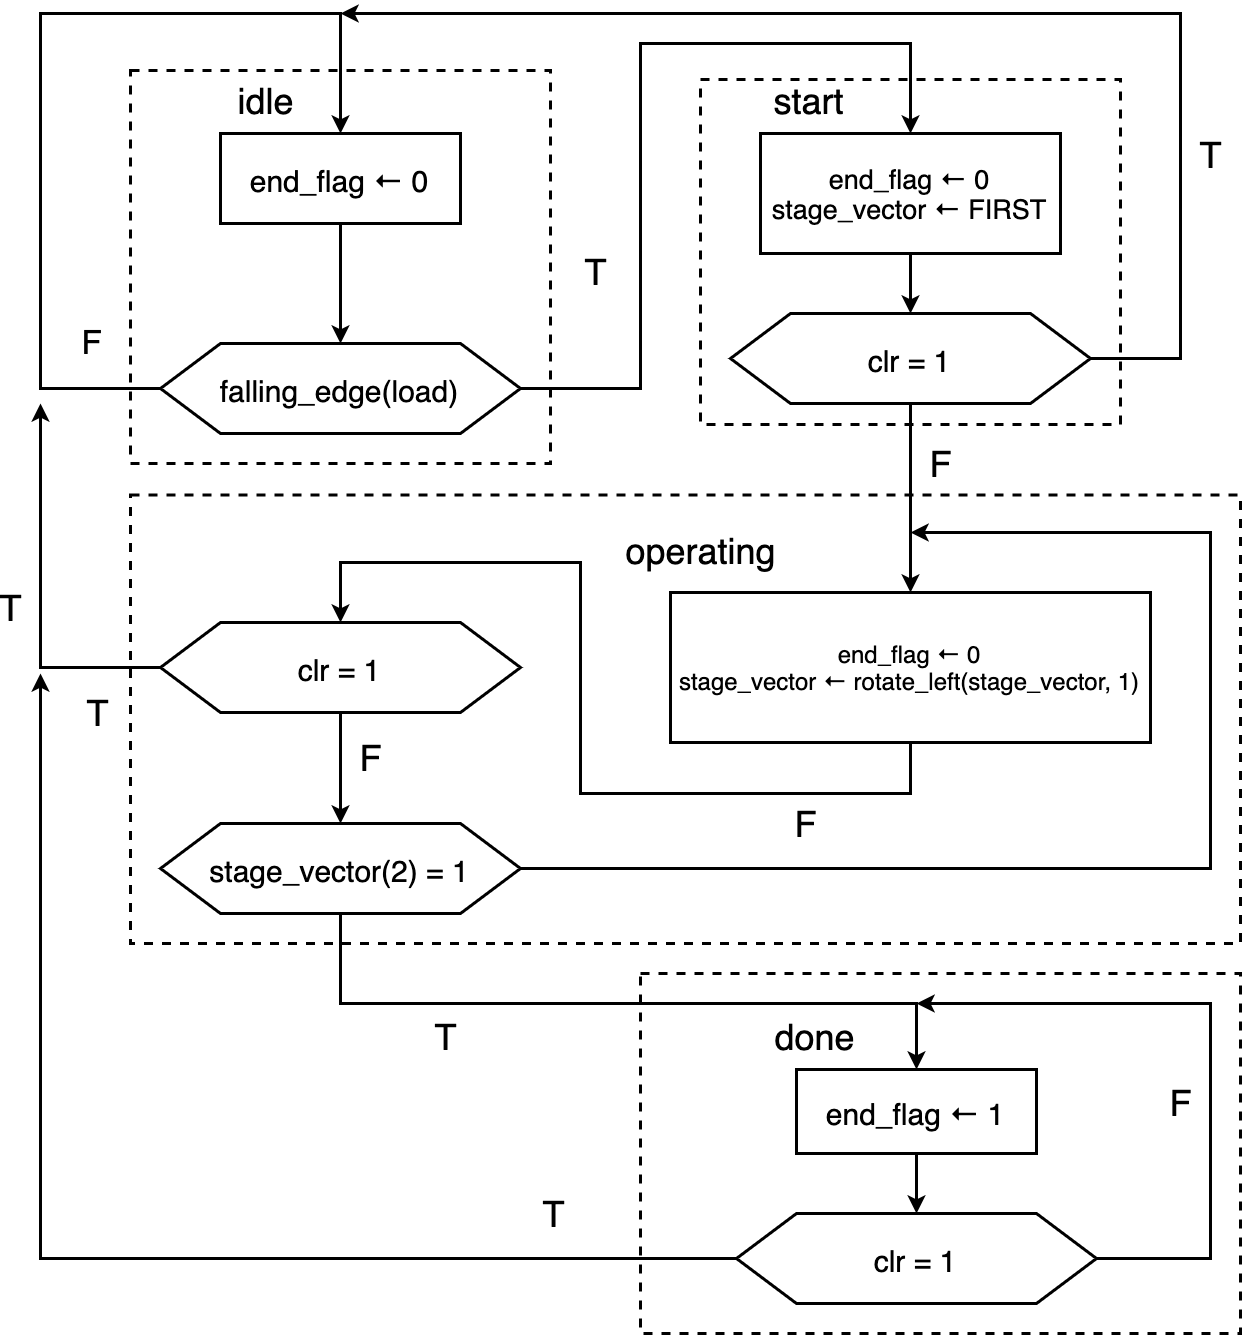
\includegraphics[width=0.6\textwidth]{./img/asmd.png}}

	\figurenote{In (b), the \textquote{stege\_vector} is a 3 bit vector signal and the \textquote{FIRST} is \textquote{001}.}
	% \figurenote{Eight code values were provided to simulate the \(extended\_pp\).}
\end{figure}

% \begin{figure*}[!ht]
% 	\centering
% 	\caption{Synthesized RTL Diagram of 4 Stages \(End\_Flag\) Generator}
% 	\includegraphics[height=0.9\textheight]{../img/end_flag_gen_rtl.png}
% 	\label{fig:end_flag_gen_rtl}
% \end{figure*}
